\section{Additional DER Background}
\label{appendix:Experiement Details}
\begin{figure}[h]
    \centering
     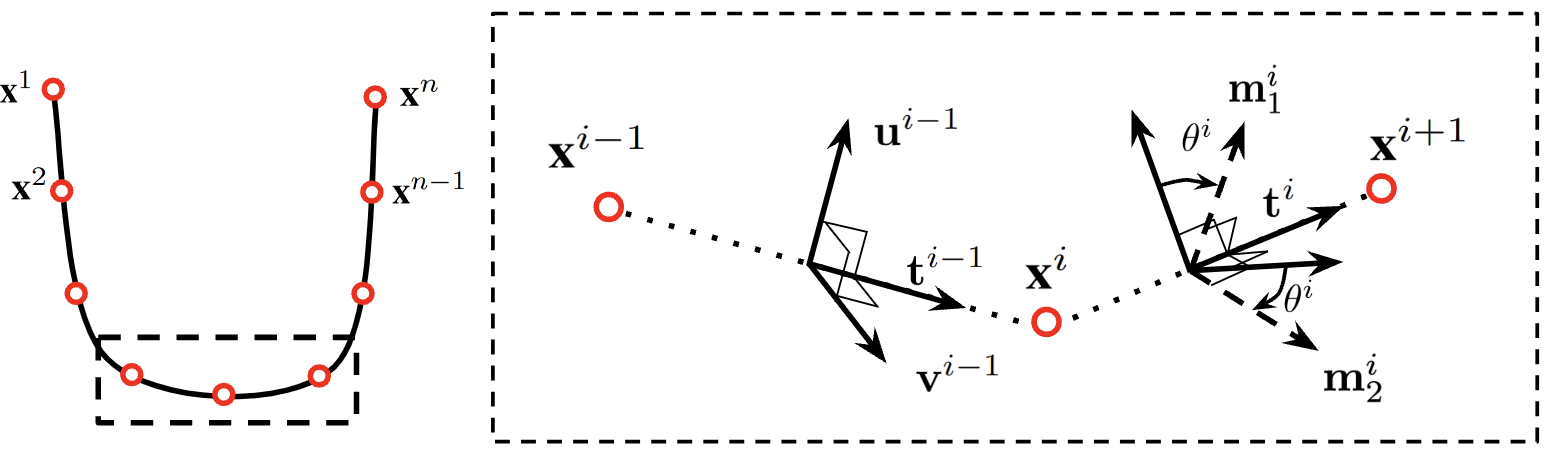
\includegraphics[width=1\textwidth]{figures/involved_coordinate_frames.png}
     \caption{An illustration of DER coordinate frames.}
    \label{fig:DER_frames}
\end{figure}

\textbf{Bishop Frame.}
To accurately approximate the potential energy of the DLO that arises due to bending or twisting, DER first assigns Bishop frames $\{\mathbf{t}^i, \mathbf{u}^i, \mathbf{v}^i\}$ as reference frame onto edge $i$.  $\mathbf{t}^i \in \mathbb{R}^{3}$ represents the unit tangent vector along edge $i$. 
The vector $\mathbf{u}^i \in \mathbb{R}^{3}$ is defined iteratively through a rotation operation $\mathbf{u}^i = \mathbf{R}^i \cdot \mathbf{u}^{i-1}$. 
This rotation is governed by a rotation matrix $\mathbf{R}^i \in \mathbb{R}^{3\times3}$, which satisfies following conditions: $\mathbf{t}^i = \mathbf{R}^i \cdot \mathbf{t}^{i-1}$ and $\mathbf{t}^{i-1} \times \mathbf{t}^i = \mathbf{R}^i \cdot (\mathbf{t}^{i-1} \times \mathbf{t}^i)$. $\mathbf{v}^i$, orthogonal to $\mathbf{t}^i$ and $\mathbf{u}^i$, is defined by $\mathbf{v}^i = \mathbf{t}^i \times \mathbf{u}^i$. 
This transportation results in the least amount of twist, making it ideal for adapting the Bishop frame as the most natural reference frame.
Further details of the Bishop frame can be found in \cite{bishopframe}.

\textbf{Material Frame.}
DER further introduces a scalar $\theta^i$ to measure the rotation of material frames $\{\mathbf{t}^i, \mathbf{m}_1^i, \mathbf{m}_2^i\}$ relative to the Bishop frame along $\mathbf{t}^\textit{i}$. $\mathbf{m}_1^i, \mathbf{m}_2^i$ are defined as following
\begin{equation}
    \mathbf{m}_1^i = \cos \theta^i \cdot \textbf{u}^i + \sin \theta^i \cdot \textbf{v}^i, \quad\mathbf{m}_2^i = -\sin \theta^i \cdot \textbf{u}^i + \cos \theta^i \cdot \textbf{v}^i.
\end{equation}
The material frames are used in \eqref{eq:opt_theta} to obtain potential energy. 
An illustration of Bishop frame and material frame can be found in Figure \ref{fig:DER_frames}. 
More relevant details can be found in \cite[Section 4]{originalDER}. 

